\documentclass[UTF8,a4paper,12pt]{ctexart}
\usepackage[left=2.5cm,right=2.5cm,top=2.6cm,bottom=2.6cm]{geometry}
\usepackage{amsmath,amssymb,booktabs,graphicx,float,array,xcolor,hyperref,tabularx,longtable,enumitem}
\graphicspath{{../figures/}}
\hypersetup{colorlinks=true,linkcolor=black,urlcolor=blue!55!black,citecolor=black}
\setlength{\parindent}{2em}
\setlength{\parskip}{0.28em}
\renewcommand{\arraystretch}{1.22}
\linespread{1.18}
\setlist{nosep,leftmargin=2.2em}
\newcommand{\dif}{\mathop{}\!\mathrm{d}}

\title{NIPT 的时点选择与胎儿异常判定}
\author{}
\date{}

\begin{document}
\maketitle

\begin{abstract}
无创产前检测的可靠性同时受检测孕周、孕妇体型和测序质量影响，附件中同一孕妇又存在多次采血或重复检测，因而不能把每条记录视为独立样本。本文分析 267 名男胎孕妇的 1082 条记录和 147 名女胎孕妇的 605 条记录，并把孕妇代码统一作为纵向随机效应、交叉验证分组和重抽样单位。

问题一对 Y 染色体浓度取对数后建立随机截距混合效应模型。孕周一次项系数为 0.0382，BMI 系数为 $-0.0224$，二者分别呈显著正、负效应；个体内相关系数达到 0.732，说明孕妇间稳定差异占主要方差。问题二将首次达到百分之四的真实时点表示为左删失、区间删失或右删失事件，以对数正态加速失效时间模型估计条件达标概率，再用动态规划形成四个连续 BMI 组。在每组至少 35 人且平均达标概率不低于九成的约束下，推荐时点依次为 13周3天、14周4天、16周2天和19周5天。

问题三加入年龄、身高、受孕方式和孕产史进行风险修正，四组时点变为 13周6天、15周2天、16周3天和19周5天；但多因素模型 AIC 为 364.38，高于仅 BMI 模型的 358.57，因此把简洁模型作为主结论、多因素模型作为边界修正。将浓度阈值由百分之三点五调至百分之四点五后，推荐时点最多改变 17 天。问题四按孕妇分组进行五折验证，逻辑回归的 ROC-AUC 为 0.826、PR-AUC 为 0.479、召回率为 0.746、特异度为 0.768，均优于传统绝对 Z 值阈值的主要筛查表现；500 次分组 Bootstrap 给出 ROC-AUC 的置信区间 $[0.760,0.878]$。模型保留了删失、不平衡和重复测量结构，所得结论仅适用于附件样本与赛题假设，不构成临床诊断建议。
\end{abstract}

\noindent\textbf{关键词：}NIPT；混合效应模型；区间删失；加速失效时间模型；动态分组；分组交叉验证

\section{问题重述}

无创产前检测（NIPT）通过分析母体外周血中的胎儿游离 DNA，对胎儿染色体非整倍体风险进行筛查。检测过早时，胎儿来源 DNA 比例可能不足；检测过晚又会压缩后续诊断和处置窗口。因此，检测时点不是单纯追求“越晚越可靠”，而是在可靠性与时间代价之间寻找可执行的平衡。既往研究表明，胎儿浓度通常随孕周增加而升高，并随孕妇 BMI 增大而降低\cite{deng,rolnik}；无信息结果也与孕周、BMI 和年龄有关\cite{gazdarica}。这些规律提供了建模方向，但本题的所有参数仍必须由附件数据估计。

题目给出男胎与女胎两个工作表。男胎可直接利用 Y 染色体浓度判断检测结果是否基本可靠，题面把 4\% 作为重要达标阈值；女胎没有 Y 染色体这一直接参照，需要综合 13、18、21 号常染色体 Z 值、X 染色体指标和测序质量变量判断异常。Z-score 是 NIPT 常用的统计量，但其准确性依赖数据处理和实验平台\cite{zhang}，因而不能不经验证地把单一阈值当作附件标签的完整生成规则。

问题一要求研究男胎 Y 染色体浓度与孕周、BMI 等因素的关系，并检验关系的显著性。问题二要求以 BMI 为主要因素划分孕妇群体，给出各组适宜的 NIPT 时点，并分析检测误差的影响。问题三要求进一步综合身高、体重、年龄等因素，重新讨论分组与时点。问题四要求对女胎染色体异常进行判定。四问分别对应纵向关系估计、删失时点决策、多因素稳健修正和不平衡分类，但共享同一个关键结构：同一孕妇的多条检测记录具有相关性。

附件中男胎有 1082 条记录、267 名孕妇，女胎有 605 条记录、147 名孕妇，平均每名孕妇分别有 4.052 和 4.116 条记录。重复记录包含多次采血、同次采血的重复检测或相近孕周的再次测量。若随机按行划分训练集和验证集，同一孕妇的个体特征会同时出现在两侧，得到过于乐观的误差。因此，本文把孕妇代码作为纵向随机效应、交叉验证分组和 Bootstrap 重抽样的共同单位。

\section{问题分析}

\subsection{问题一的关系识别}

Y 染色体浓度为正且呈右偏分布，原始尺度上的方差随均值变化。若直接拟合普通最小二乘模型，不仅残差同方差假设较弱，而且会忽略同一孕妇多次测量的相关性。我们先对浓度取对数，使乘性差异转化为加性差异；再为每名孕妇引入随机截距，表示无法由年龄、BMI 和质量变量解释的稳定个体差异。固定效应中保留孕周二次项，用于容纳浓度随孕周的非线性增长；加入孕周与 BMI 的交互项，用于检验高 BMI 是否改变孕周增速。模型输出既包括系数及显著性，也包括个体内相关系数和按孕妇分组的预测误差。

问题一的基线是带聚类稳健标准误的固定效应回归。该基线能修正部分标准误，却不能直接分解孕妇层方差，也无法给出随机效应解释。树回归可以拟合更复杂的非线性，但对“方向、显著性、个体异质性占比”三个核心问题回答较弱。因此，随机截距混合效应模型作为主模型，固定效应回归只用于组外预测基线，残差图和 Q-Q 图用于检查模型边界。

\subsection{问题二的删失时点与分组决策}

每名孕妇的真实首次达标孕周通常没有被连续观察。若第一次检测已经达到 4\%，只能知道真实达标时点不晚于该次检测，这属于左删失；若先未达标、后达标，则真实时点落在两次检测之间，属于区间删失；若所有检测均未达标，则只能知道真实时点晚于最后一次检测，属于右删失。附件中三类孕妇分别为 218、42 和 7 人。把第一次观测到达标的孕周直接视为真实时点，会对 218 名左删失孕妇产生系统性偏晚估计，因此需要以删失似然建模。

题面要求给出 BMI 分组和最佳时点。我们把“最佳”明确为：在某组预测达标比例首次达到 90\% 时选择最早孕周。这个定义把可靠性写成硬约束，把时间写成单调代价，避免人为拼接难解释的风险权重。BMI 分组还需满足连续、互斥、覆盖样本且每组容量足够。我们先由 AFT 模型计算每名孕妇的条件 90\% 达标分位数，再用动态规划寻找组内同质、组间有别的四段连续区间，最后在每天粒度的孕周网格上搜索满足概率约束的最早时点。

\subsection{问题三的多因素修正}

问题三要求考虑身高、体重、年龄等因素。BMI 已由体重和身高共同计算，若同时机械加入 BMI、身高、体重，容易形成强共线性。为保持参数可解释性，主路线保留 BMI 和身高，而不再单独加入体重；再加入年龄、受孕方式、怀孕次数和生产次数。所有变量都必须在检测决策前可获得。Z 值、GC 比例、读段数和 Y 浓度属于检测后信息，虽然能解释是否达标，却不能用于决定“何时去检测”，否则会产生时序泄漏。

多因素模型不应因为变量更多就被视为更好。本文预先规定用 AIC 比较仅 BMI 与多因素 AFT：若多因素 AIC 降低，则说明复杂度得到似然改善补偿；若 AIC 上升，则只把多因素结果作为风险修正和异质性描述。同时，把达标阈值从 4\% 改为 3.5\% 和 4.5\%，重新构造全部删失区间、重新拟合模型并重新计算时点，使测量误差从原始判定一直传播到最终建议。

\subsection{问题四的不平衡异常判定}

女胎数据中异常记录为 67 条，阳性率约 11.1\%。在这种类别不平衡下，准确率会被大量正常记录主导。模型评价必须同时报告 ROC-AUC、PR-AUC、召回率、特异度和 F1，并给出混淆矩阵。传统规则取 $\max(|Z_{13}|,|Z_{18}|,|Z_{21}|)\ge3$ 作为异常基线；主模型采用标准化逻辑回归；随机森林和直方图梯度提升作为非线性对照。四个模型使用同一组按孕妇锁定的五折划分，避免验证设计差异影响比较。

逻辑回归的优势是系数方向可解释，且在小阳性样本下比复杂集成模型更稳定。随机森林可捕捉阈值和交互，梯度提升可刻画连续非线性，但两者若在召回率和 PR-AUC 上没有改善，就不应仅凭复杂度成为主模型。最终还以孕妇为单位做 500 次 Bootstrap；每次抽到某名孕妇时，整组重复记录一并进入样本，从而保留组内相关结构。

\section{模型假设}

\textbf{假设 1：}孕妇代码唯一标识同一受试者。同一代码下的多次检测共享稳定个体差异，不同孕妇之间相互独立。该假设是随机截距、分组交叉验证和分组 Bootstrap 的共同基础。

\textbf{假设 2：}男胎 Y 染色体浓度第一次越过 4\% 后，真实“首次达标时点”可由相邻未达标和达标观测夹住。短期测量波动可能造成局部回落，但题目关注的是达到基本可靠水平的时点，因此以首次观测越过阈值构造事件区间。

\textbf{假设 3：}条件于协变量后，首次达标时间的对数近似服从正态分布。该假设不被当作医学定律，只是 AFT 主模型的工作分布；通过阈值扰动、AIC 比较和覆盖约束检查评估其稳健性。

\textbf{假设 4：}在 10 至 25 周的题面范围内，组平均达标概率随孕周总体不下降。对数正态 AFT 自然满足这一单调性，因此推荐时点搜索不会出现“晚一周反而更不可靠”的逻辑冲突。

\textbf{假设 5：}检测前人口学变量的记录误差相对有限；女胎缺失的一个 BMI 可在每个训练折中用中位数填补。缺失值填补参数只由训练折估计，避免验证信息进入训练过程。

\textbf{假设 6：}女胎“染色体的非整倍体”字段非空表示异常，空白表示正常。出生后的“胎儿是否健康”不替代该标签，因为它是事后变量，且健康结局与筛查标签不是同一概念。

\textbf{假设 7：}附件样本的检测平台和字段口径在记录间保持一致。若平台、批次或实验室流程改变，需要重新校准模型截距、阈值和概率，不可直接沿用本文数值。

\textbf{假设 8：}模型结论只面向题目附件覆盖的人群。附件 BMI 中位数约为 31.5，明显偏向高 BMI 人群；对一般孕妇或临床人群的外推必须有新的代表性样本支持。

\section{符号说明}

\begin{table}[H]
\centering
\caption{主要符号、含义与单位}
\small
\begin{tabularx}{0.96\textwidth}{cXc}
\toprule
符号 & 含义 & 单位 \\
\midrule
$Y_{ij}$ & 第 $i$ 名孕妇第 $j$ 次检测的男胎 Y 染色体浓度 & 比例 \\
$W_{ij}$ & 第 $i$ 名孕妇第 $j$ 次检测孕周 & 周 \\
$B_i$ & 第 $i$ 名孕妇代表性 BMI & kg/m$^2$ \\
$u_i$ & 孕妇层随机截距 & 无量纲 \\
$T_i$ & 第 $i$ 名孕妇首次达到浓度阈值的真实孕周 & 周 \\
$(L_i,U_i]$ & 首次达标时点的删失区间 & 周 \\
$\mu_i$ & AFT 模型中 $\log T_i$ 的条件均值 & 无量纲 \\
$\sigma$ & AFT 对数时间尺度参数 & 无量纲 \\
$q_i$ & 第 $i$ 名孕妇条件 90\% 达标分位数 & 周 \\
$c_k$ & 第 $k$ 个 BMI 分组边界 & kg/m$^2$ \\
$t_k^*$ & 第 $k$ 组推荐检测孕周 & 周 \\
$p_i$ & 女胎第 $i$ 条记录的预测异常概率 & 比例 \\
$z_{0.9}$ & 标准正态分布的 0.9 分位数 & 无量纲 \\
\bottomrule
\end{tabularx}
\end{table}

\section{数据预处理}

\subsection{字段解析与质量检查}

原始孕周以“周数 w 加天数”的字符串给出。我们将 $aw+b$ 统一换算为 $a+b/7$ 周，保留到计算精度，不在模型拟合前四舍五入。男胎只有 1 条孕周无法解析，该记录不能参与时点和纵向模型；女胎孕周均可解析。怀孕次数中可能混有文字说明，采用正则提取首个整数；受孕方式编码为自然受孕与非自然受孕二元变量。

附件没有完全相同的重复行，但同一孕妇存在多次记录。本文不把这些记录当作数据重复而删除，因为它们提供了纵向变化和测量波动信息。男胎平均每人 4.052 条记录，女胎平均每人 4.116 条记录；多数孕妇恰有 4 条记录，少数有 1 至 9 条。若简单按行加权，记录较多的孕妇会对模型贡献更大，因此推断模型显式加入随机效应，验证和重抽样均锁定孕妇组。

\begin{table}[H]
\centering
\caption{数据规模与缺失概览}
\small
\begin{tabular}{lrrrrrr}
\toprule
工作表 & 记录数 & 孕妇数 & 平均重复 & 孕周缺失 & BMI缺失 & 标签阳性率 \\
\midrule
男胎 & 1082 & 267 & 4.052 & 1 & 0 & 0.866 \\
女胎 & 605 & 147 & 4.116 & 0 & 1 & 0.111 \\
\bottomrule
\end{tabular}
\end{table}

女胎只有 1 个 BMI 缺失。分类模型使用流水线在每个训练折内计算中位数并填补，再进行标准化或树模型拟合。这样既保留该样本，又避免用全数据中位数把验证折信息带入训练。Y 染色体浓度、异常标签和用于主要模型的 Z 值没有采用外部数据补齐。极端 BMI 和极端浓度可能是真实高风险个体，因此不以固定箱线规则删除；其影响通过对数变换、稳健验证和适用范围说明控制。

如图~\ref{fig:data_profile} 所示，四个最影响模型设计的数据特征分别是 BMI 偏态、检测孕周多峰、受试者内重复和女胎标签不平衡。男胎 BMI 主要集中在 28 至 36，右尾延伸到 46.9；检测孕周在 10 至 25 周内呈多峰分布，反映不同复检安排；每名孕妇多为 4 次记录；女胎异常类别远少于正常类别。这些特征分别对应外推限制、删失建模、分组验证和不平衡指标选择。

\begin{figure}[H]
\centering
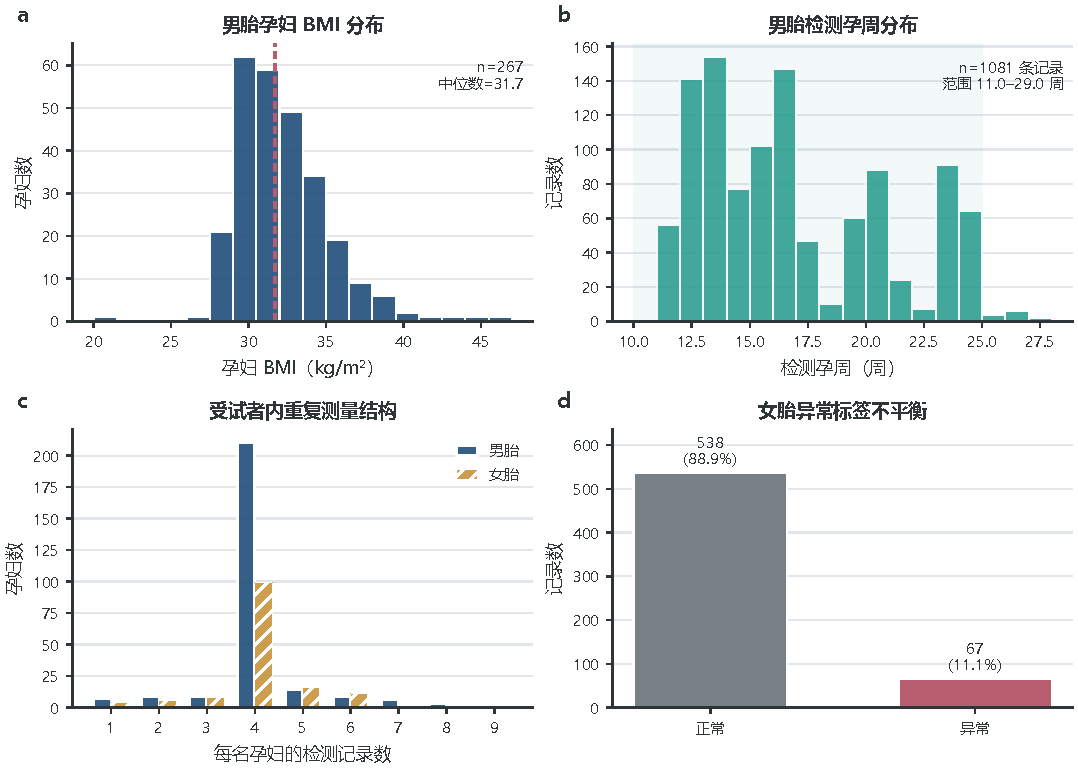
\includegraphics[width=0.96\textwidth]{data_profile_distribution.pdf}
\caption{样本分布、重复测量结构与女胎标签不平衡}\label{fig:data_profile}
\end{figure}

\subsection{记录层、孕妇层与决策层的区分}

附件的一行表示一次检测记录，但问题二、三的推荐对象是一名孕妇，问题四的验证对象也应是尚未见过的孕妇。若不区分这三个层级，会出现两类偏差。其一，记录较多的孕妇在目标函数中被重复计权，使其个人测量习惯被误当成人群规律；其二，同一孕妇的年龄、身高、受孕方式等稳定变量同时进入训练折和验证折，模型即使没有学到可迁移关系，也能借助近似重复的特征获得较高分数。为此，本文在描述原始浓度变化时保留记录层数据，在构造首次达标区间和 BMI 分组时压缩到孕妇层，在计算最终推荐时点时再汇总到分组决策层。三层对象不同，但都由孕妇代码连接，任何统计量都明确其分母是记录数还是孕妇数。

男胎纵向模型使用 1081 条孕周可解析记录，因为每次测量都携带新的浓度信息；AFT 时点模型则使用 267 名孕妇，每人只贡献一个删失区间和一组检测前协变量。对于在多次检测间不完全恒定的 BMI，取该孕妇有效记录的中位数，降低单次录入或测量波动的影响。年龄、身高、受孕方式和孕产史同样先检查孕妇内一致性，再形成孕妇层特征。这样处理后，AFT 似然中的每一项对应一名独立受试者，动态分组的最小容量 35 也明确指 35 名孕妇，而不是 35 条可能来自少数人的记录。

女胎分类需要在记录层输出判定，因为标签与一次检测对应；但五折划分在孕妇层生成。设第 $i$ 名孕妇的记录集合为 $\mathcal R_i$，则任一折的训练集合和验证集合都满足
\begin{equation}
\left(\bigcup_{i\in\mathcal I_{\mathrm{train}}}\mathcal R_i\right)
\cap
\left(\bigcup_{i\in\mathcal I_{\mathrm{valid}}}\mathcal R_i\right)=\varnothing,
\qquad
\mathcal I_{\mathrm{train}}\cap\mathcal I_{\mathrm{valid}}=\varnothing.
\label{eq:groupsplit}
\end{equation}
该条件比随机划分记录更严格，也更接近模型面对新孕妇时的使用情景。类别比例只能在满足组隔离后尽量平衡，不能为了让每折阳性数完全相同而拆散同一孕妇。

异常值处理遵循“先核查、后稳健化、慎删除”。BMI 高值、浓度高值或低值都可能对应题目刻意覆盖的特殊人群，若仅因偏离箱线范围而删除，会把最需要讨论的高 BMI 风险区抹去。因此，只删除无法转换为数值且没有可恢复信息的记录；对正浓度使用对数变换，对连续特征在训练折内标准化，对树模型保留原尺度。最终还比较边际相关、混合模型系数方向和分组时点顺序，若三者出现不可解释的方向冲突，再回查原始记录，而不是用删点制造一致性。

\subsection{变量时序与标签构造}

时点模型只允许使用检测前可获得的 BMI、年龄、身高、受孕方式和孕产史。Y 浓度仅用于构造达标事件，不能反向作为推荐时点的预测变量；GC 含量、读段数和 Z 值在抽血测序后才得到，同样不能进入问题二、三的检测前决策。问题四本身发生在检测后，因此可以使用 Z 值和测序质量变量。出生健康字段属于更晚的结局，仅用于检查数据口径，不作为异常标签或预测变量。

对男胎，以 $Y_{ij}\ge0.04$ 定义该次检测达标。对每名孕妇按孕周排序后构造区间：若第一次记录即达标，置 $L_i=0$、$U_i=W_{i1}$；若第 $r$ 次首次达标，置 $L_i=W_{i,r-1}$、$U_i=W_{ir}$；若始终未达标，置 $L_i=W_{im}$、$U_i=\infty$。同一孕周的重复检测先按孕周和结果排序，不虚构比天级更细的真实先后次序。

对女胎，以“染色体的非整倍体”字段是否非空构造二元标签。传统 Z 基线只使用 13、18、21 号染色体的绝对 Z 值；学习模型还加入 X 染色体浓度与 Z 值、各染色体 GC 含量、原始和唯一比对读段数、比对比例、重复和过滤比例、BMI、年龄与孕周。所有数值指标均由训练折内的预处理器处理。

\section{模型建立与求解}

\subsection{问题一：随机截距混合效应模型}

令中心化后的孕周、BMI、年龄、GC 含量和过滤比例分别为 $W^c_{ij}$、$B^c_{ij}$、$A^c_{ij}$、$G^c_{ij}$ 和 $F^c_{ij}$。对数浓度模型写为
\begin{equation}
\log Y_{ij}=\beta_0+\beta_1W^c_{ij}+\beta_2(W^c_{ij})^2+\beta_3B^c_{ij}+\beta_4W^c_{ij}B^c_{ij}+\beta_5A^c_{ij}+\beta_6G^c_{ij}+\beta_7F^c_{ij}+u_i+\varepsilon_{ij}.
\label{eq:mixed}
\end{equation}
随机项满足
\begin{equation}
u_i\sim N(0,\tau^2),\qquad \varepsilon_{ij}\sim N(0,\sigma_e^2),\qquad u_i\perp\varepsilon_{ij}.
\label{eq:random}
\end{equation}
对数变换使系数具有近似相对变化解释。例如其他变量不变时，BMI 增加 1 个单位对应浓度乘以 $\exp(\beta_3)$；孕周效应则由一次项、二次项和交互项共同决定。所有连续变量先中心化，降低一次项与二次项、主效应与交互项之间的数值相关。

个体内相关系数定义为
\begin{equation}
\mathrm{ICC}=\frac{\tau^2}{\tau^2+\sigma_e^2},
\label{eq:icc}
\end{equation}
用于衡量同一孕妇两次观测的相关程度。边际和条件决定系数分别记为
\begin{equation}
R_m^2=\frac{V_f}{V_f+\tau^2+\sigma_e^2},\qquad
R_c^2=\frac{V_f+\tau^2}{V_f+\tau^2+\sigma_e^2},
\label{eq:r2}
\end{equation}
其中 $V_f$ 为固定效应预测值的方差。$R_m^2$ 衡量可观测固定变量的解释力，$R_c^2$ 还包括孕妇随机差异。

\subsubsection{参数估计、比较基准与效应解释}

对第 $i$ 名孕妇的全部观测记为向量 $\boldsymbol y_i$，固定效应设计矩阵记为 $X_i$。在随机截距结构下，其边际协方差矩阵为
\begin{equation}
V_i=\tau^2\boldsymbol 1\boldsymbol 1^\top+\sigma_e^2 I,
\qquad
\boldsymbol y_i\sim N(X_i\beta,V_i).
\label{eq:mixedcov}
\end{equation}
矩阵的非对角元均为 $\tau^2$，直接表示同一孕妇两次对数浓度的共同成分；不同孕妇之间的协方差为零。最大似然估计同时选择固定效应 $\beta$、孕妇层方差 $\tau^2$ 和记录层方差 $\sigma_e^2$，而不是先估计每名孕妇均值再做回归。后一种两阶段方法会让只有一次检测和有多次检测的孕妇受到相同处理，丢失测量次数带来的精度差异，也难以正确传播均值估计误差。

选择孕周二次项而不是高阶多项式，依据是解释与稳定性的平衡。一次项只能给出恒定增速，难以容纳 10 至 25 周内的轻微弯曲；三次以上多项式在区间端点容易振荡，而且问题并不要求构造长期生理曲线。中心化后，$\beta_1$ 表示 BMI、年龄和质量变量处于样本中心时的局部孕周效应，$\beta_3$ 表示中心孕周附近 BMI 每增加一个单位的条件效应。孕周的边际导数为
\begin{equation}
\frac{\partial E(\log Y_{ij}\mid u_i)}{\partial W_{ij}}
=\beta_1+2\beta_2W^c_{ij}+\beta_4B^c_{ij},
\label{eq:weekderivative}
\end{equation}
因此不能只根据一次项讨论所有孕周的增速。交互项的 $p$ 值为 0.326，说明在本样本中没有足够证据把高 BMI 解释为改变增长斜率；更稳妥的表述是高 BMI 主要使曲线整体下移。

显著性检验的零假设为相应固定效应系数等于零，采用估计值与渐近标准误构造双侧 $z$ 检验。统计显著不等于个体预测准确：孕周和 BMI 系数可以在大量重复记录中被稳定识别，但新孕妇的随机截距未知，仍会导致较宽预测误差。为区分这两种问题，本文同时报告条件拟合和组外预测。条件拟合把估计的 $u_i$ 用于已见孕妇，回答“模型能否描述已有纵向轨迹”；组外验证把待预测孕妇的随机效应置为总体均值零，回答“仅凭检测前与质量变量能否预测新个体”。二者用途不同，不能用较高的条件 $R_c^2$ 代替组外性能。

固定效应回归作为组外基准时，仍按孕妇划分折次，并在每一训练折重新估计中心化常数和系数。若先用全样本均值中心化，虽然数值影响通常较小，却会让验证折的分布信息提前进入训练。本文所有变换均在训练数据上确定，验证折只应用既定变换。对于问题一，分组交叉验证的目的不是筛选大量超参数，而是揭示“总体关联显著”和“个体浓度难预测”可以同时成立，从而限定模型结论的层级。

混合模型按最大似然估计，求解步骤如下：
\begin{enumerate}
  \item 删除无法解析孕周或主变量缺失的记录，对浓度取自然对数并中心化连续变量；
  \item 先拟合固定效应结构，再以孕妇代码加入随机截距，使用 L-BFGS 迭代至似然收敛；
  \item 由估计协方差计算系数标准误、$z$ 统计量和 95\% 置信区间；
  \item 计算 ICC、$R_m^2$、$R_c^2$，并以五折 GroupKFold 检验新孕妇固定效应预测误差；
  \item 绘制拟合关系、拟合值--残差图与 Q-Q 图，检查非线性、异方差和尾部偏离。
\end{enumerate}

\begin{table}[H]
\centering
\caption{问题一混合效应模型的关键固定效应}
\small
\begin{tabular}{lrrrr}
\toprule
变量 & 系数 & 标准误 & $p$ 值 & 95\% 置信区间 \\
\midrule
孕周一次项 & 0.0382 & 0.0026 & $3.23\times10^{-48}$ & [0.0331, 0.0434] \\
孕周二次项 & 0.0024 & 0.0005 & $8.35\times10^{-6}$ & [0.0013, 0.0034] \\
BMI & -0.0224 & 0.0074 & 0.0026 & [-0.0370, -0.0078] \\
孕周$\times$BMI & 0.0007 & 0.0007 & 0.3257 & [-0.0007, 0.0020] \\
年龄 & -0.0124 & 0.0071 & 0.0785 & [-0.0263, 0.0014] \\
GC 含量 & 6.9504 & 2.6787 & 0.0095 & [1.7002, 12.2005] \\
\bottomrule
\end{tabular}
\end{table}

孕周一次项显著为正，BMI 系数显著为负；交互项不显著，说明附件不足以支持“BMI 显著改变孕周增长斜率”的强结论。年龄在 5\% 水平不显著，GC 含量显著，提示实验质量变量会影响单次浓度。ICC 为 0.7318，$R_m^2=0.1440$，$R_c^2=0.7705$。固定变量只能解释约 14.4\% 的总变异，加入孕妇随机差异后解释率大幅提高，这正是不能把重复记录视为独立样本的数值证据。

如图~\ref{fig:q1_relation} 所示，左侧以记录密度为底图并叠加不同 BMI 下的模型曲线，右侧给出 BMI 分箱中位数、四分位距以及不同孕周的条件预测。相同孕周下高 BMI 曲线整体较低；观测四分位距仍较宽，与高 ICC 一致。虚线为 4\% 阈值，它只用于问题二、三的可靠性事件，不表示浓度越高越能直接诊断染色体异常。

\begin{figure}[H]
\centering
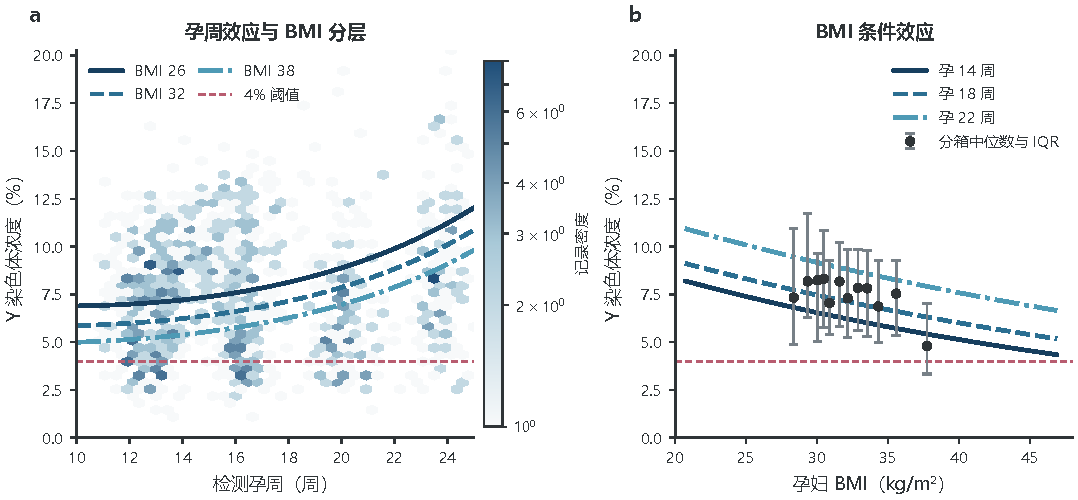
\includegraphics[width=0.96\textwidth]{q1_relationships.pdf}
\caption{孕周、BMI 与男胎 Y 染色体浓度关系}\label{fig:q1_relation}
\end{figure}

\subsection{问题二：区间删失 AFT 与动态 BMI 分组}

设 $T_i$ 为第 $i$ 名孕妇的真实首次达标孕周，观测只给出 $T_i\in(L_i,U_i]$。仅 BMI 的对数正态 AFT 模型为
\begin{equation}
\log T_i=\alpha_0+\alpha_1\widetilde B_i+\sigma\epsilon_i,qquad \epsilon_i\sim N(0,1),
\label{eq:aft}
\end{equation}
其中 $\widetilde B_i$ 是标准化 BMI。记 $\mu_i=\alpha_0+\alpha_1\widetilde B_i$，标准正态分布函数为 $\Phi$。单个样本对似然的贡献为
\begin{equation}
\mathcal L_i=
\begin{cases}
\Phi\!\left(\dfrac{\log U_i-\mu_i}{\sigma}\right), & L_i=0,\\[6pt]
\Phi\!\left(\dfrac{\log U_i-\mu_i}{\sigma}\right)-
\Phi\!\left(\dfrac{\log L_i-\mu_i}{\sigma}\right), & 0<L_i<U_i<\infty,\\[6pt]
1-\Phi\!\left(\dfrac{\log L_i-\mu_i}{\sigma}\right), & U_i=\infty.
\end{cases}
\label{eq:likelihood}
\end{equation}
三种似然项分别回答不同的信息边界。左删失者只说明 $T_i$ 落在第一次检测之前，其贡献是累积分布函数值；区间删失者提供上下界，其贡献是两个累积分布函数之差；右删失者只说明事件尚未发生，其贡献是生存概率。直接删除 7 名右删失者会把最晚达标的人群排除，系统性提前推荐时点；把 218 名左删失者的首次检测周当作精确事件，又会把本来可能更早的达标时点向后推。区间删失似然在不虚构事件日期的条件下使用全部 267 名孕妇，是时点估计的核心。

为避免两个累积分布函数非常接近时发生浮点下溢，计算中对每项概率设置极小的数值下界，并在对数尺度累加。尺度参数写成 $\sigma=\exp(\eta)$，优化变量 $\eta\in\mathbb R$ 不受约束，从而自动满足 $\sigma>0$。初值由首次观测达标周的对数回归近似给出，但最终估计使用完整删失似然。求解完成后同时检查优化器成功标记、梯度大小、尺度为正及所有个体概率位于零和一之间；若任一检查失败，便不进入后续分组。

模型通过最小化 $-\sum_i\log\mathcal L_i$ 求解，并以 $\log\sigma$ 作为优化变量保证尺度参数为正。给定孕妇协变量，其在孕周 $t$ 前达到阈值的概率为
\begin{equation}
P(T_i\le t\mid X_i)=\Phi\!\left(\frac{\log t-X_i^\top\widehat\alpha}{\widehat\sigma}\right).
\label{eq:probability}
\end{equation}

每名孕妇条件 90\% 达标分位数为
\begin{equation}
q_i=\exp\!\left(X_i^\top\widehat\alpha+\widehat\sigma z_{0.9}\right).
\label{eq:quantile}
\end{equation}
将孕妇按 BMI 从小到大排序。若第 $a$ 至第 $b$ 名孕妇构成一组，定义组内损失
\begin{equation}
D(a,b)=\sum_{i=a}^{b}(q_i-\bar q_{a:b})^2.
\label{eq:segmentloss}
\end{equation}
四组边界的决策变量为 $0=c_0<c_1<c_2<c_3<c_4=n$，目标函数和约束写为
\begin{align}
\min_{c_1,c_2,c_3}\quad & \sum_{k=1}^{4}D(c_{k-1}+1,c_k), \label{eq:dpobjective}\\
\text{s.t.}\quad & c_k-c_{k-1}\ge35,\quad k=1,2,3,4, \nonumber\\
& B_{c_k}<B_{c_k+1},\quad k=1,2,3. \label{eq:dpconstraints}
\end{align}
第二个约束禁止在相同 BMI 值内部切分。动态规划状态 $F(k,j)$ 表示前 $j$ 名孕妇分成 $k$ 组的最小损失，递推式为
\begin{equation}
F(k,j)=\min_{h}\{F(k-1,h)+D(h+1,j)\},
\label{eq:dprecursion}
\end{equation}
其中 $h$ 同时满足最小组容量和不同 BMI 边界要求。回溯最优前驱即可得到三个切点。

动态规划的必要性来自边界联动。若依次寻找三个局部最优切点，前一个切点会改变后续可用样本和最小容量，贪心结果不保证总组内损失最小。对排序后的前缀和
\begin{equation}
S_1(j)=\sum_{i=1}^{j}q_i,qquad S_2(j)=\sum_{i=1}^{j}q_i^2,
\label{eq:prefix}
\end{equation}
任一区段损失可在常数时间计算为
\begin{equation}
D(a,b)=S_2(b)-S_2(a-1)-
\frac{[S_1(b)-S_1(a-1)]^2}{b-a+1}.
\label{eq:fastloss}
\end{equation}
因此不必对每个候选区段重复遍历孕妇。四组情形的时间复杂度约为 $O(Kn^2)$，其中 $K=4$、$n=267$，在保留全局最优性的同时计算量很小。相同 BMI 不能被分到相邻两组，否则同一个 BMI 会对应两套建议，实际执行时无法判别；故只在相邻 BMI 不同的位置允许转移。

损失函数使用条件九成分位数 $q_i$，而不是 BMI 本身或条件均值。按 BMI 等距切分只能得到整齐区间，不能保证同组孕妇具有相近的可靠时点；按 $q_i$ 直接聚类又可能产生 BMI 不连续的组，使规则难以执行。本文先按 BMI 固定顺序，再最小化 $q_i$ 的组内离差，相当于在“可解释的一维连续规则”内寻找最同质的时点分组。最小组容量 35 约占 267 名孕妇的八分之一，既防止极小尾组产生偶然切点，也允许高 BMI 尾部单独成组。

分组目标与时点目标彼此分开：动态规划先决定哪些孕妇共用一条规则，机会约束再决定该组最早何时检测。若把两者合成一个加权和，时间损失和不达标风险的权重单位不同，结论会依赖任意系数。当前两阶段形式把九成可靠性作为硬条件，时间只在可行解中最小化。对任意组，$\bar P_k(t)$ 随 $t$ 单调不降，因此天级搜索得到的第一个可行点具有清晰的最早性；把周数换成整数天后再输出“周加天”，避免十进制孕周被误读为十进制天数。

分组后，对第 $k$ 组 $G_k$ 定义组平均达标概率
\begin{equation}
\bar P_k(t)=\frac{1}{|G_k|}\sum_{i\in G_k}P(T_i\le t\mid X_i),qquad
t_k^*=\min\{t\in\mathcal T:\bar P_k(t)\ge0.90\},
\label{eq:recommend}
\end{equation}
其中 $\mathcal T$ 为 10 至 25 周、步长 1 天的搜索网格。这个规则直接把可靠性写成机会约束，并在约束满足后选择最早时间。

求解流程为：
\begin{enumerate}
  \item 按孕妇和孕周排序，构造左删失、区间删失和右删失边界；
  \item 标准化 BMI，最大化区间删失似然并检查优化收敛；
  \item 计算每名孕妇的条件 90\% 分位数 $q_i$，预计算所有可行区段损失；
  \item 用动态规划求四组连续边界，回溯得到 BMI 区间；
  \item 在天级孕周网格上计算每组平均达标概率，输出最早满足 0.90 的时点；
  \item 核对每组人数、概率约束和检测窗口，任何约束不满足时不输出推荐。
\end{enumerate}

\begin{table}[H]
\centering
\caption{问题二的 BMI 分组和推荐时点}
\small
\begin{tabular}{ccccc}
\toprule
组别 & BMI 区间 & 孕妇数 & 推荐时点 & 预测达标比例 \\
\midrule
1 & [20.70, 30.19] & 70 & 13周3天 & 0.9016 \\
2 & [30.29, 32.50] & 89 & 14周4天 & 0.9003 \\
3 & [32.56, 35.35] & 73 & 16周2天 & 0.9020 \\
4 & [35.38, 46.88] & 35 & 19周5天 & 0.9016 \\
\bottomrule
\end{tabular}
\end{table}

四组推荐时点随 BMI 单调推迟，符合“高 BMI 对应较低胎儿浓度”的问题一结论。组 4 虽覆盖较宽 BMI 范围，但人数恰为最小容量 35，继续细分会显著降低稳定性。各组推荐点的预测达标比例刚超过 0.90，这是“最早可行”规则的自然结果，不是刻意把概率调到接近 0.90。

\subsection{问题三：多因素风险修正与模型比较}

多因素 AFT 使用 BMI、年龄、身高、非自然受孕指示变量、怀孕次数和生产次数。设标准化协变量向量为 $X_i$，模型为
\begin{equation}
\log T_i=\gamma_0+\gamma_1\widetilde B_i+\gamma_2\widetilde A_i+\gamma_3\widetilde H_i+
\gamma_4 I_i^{\mathrm{IVF}}+\gamma_5\widetilde G_i+\gamma_6\widetilde P_i+\sigma_3\epsilon_i.
\label{eq:aftmulti}
\end{equation}
删失似然、动态分组和推荐规则与问题二相同。为了惩罚无效复杂度，以
\begin{equation}
\mathrm{AIC}=2K-2\log\widehat{\mathcal L}
\label{eq:aic}
\end{equation}
比较模型，其中 $K$ 为自由参数数目。仅 BMI 模型的负对数似然为 176.28、AIC 为 358.57；多因素模型负对数似然降至 174.19，但参数增多后 AIC 升至 364.38。似然略有改善不足以抵消复杂度，因此问题二模型仍是简洁主基线，问题三模型用于描述风险异质性和给出修正后的分组建议。

\subsubsection{协变量选择与风险修正规则}

体重、身高和 BMI 之间满足近似确定关系 $\mathrm{BMI}=\mathrm{weight}/\mathrm{height}^2$。三者同时标准化后进入线性预测子，会使某个系数的符号高度依赖另两个变量，也会扩大标准误。题目虽要求考虑身高、体重、年龄等因素，但“考虑”不等于必须把所有派生量机械并列。本文以 BMI 表示体重相对身高的总体体型效应，另保留身高捕捉同一 BMI 下体格差异，舍去单独体重项。怀孕次数与生产次数分别表示既往妊娠经历和实际分娩经历，不能互相替代；受孕方式以二元变量进入，避免给类别强行赋连续距离。

所有连续变量在孕妇层标准化，使 AFT 系数表示协变量增加一个样本标准差对对数时点的条件影响。标准化只改善尺度和优化稳定性，不改变预测时点。类别变量保持零一编码，缺失值处理参数由训练或拟合样本确定。由于本问最终仍要输出 BMI 区间，其他协变量并不直接形成多维规则，而是先改变每名孕妇的条件分位数 $q_i$，再由动态规划观察这些风险修正是否足以移动 BMI 边界。这种做法兼顾了题目对多因素的要求与最终规则的可执行性。

AIC 比较表达的是同一批删失观测下的相对信息损失，而非绝对预测准确率。多因素模型的负对数似然改善 2.09，但增加五个左右自由参数，惩罚后 AIC 反而上升 5.81。按常用解释，这一结果不支持以复杂模型替代仅 BMI 模型。它仍有两项价值：一是检验最高风险组是否对协变量扩展稳定；二是指出中间 BMI 人群可能因年龄、身高和孕产史而重新分配。故本文把问题三结果称为“风险修正”，不称为“性能提升”。

问题三的四组边界仍要求覆盖全样本、相互不重叠并满足最小容量。某个实际 BMI 落在表格显示的小数间隙时，是因为样本中不存在该区间的观测值；实施时可把相邻观测值中点作为连续分界。例如相邻端点 31.40 与 31.41 之间不存在训练孕妇，规则可约定 BMI 不高于 31.40 归入前组，高于该值归入后组。对边界附近的测量误差，不应把 0.01 的显示精度理解成生理突变，应结合相邻组时点和阈值敏感性做保守选择。

\begin{table}[H]
\centering
\caption{问题三多因素修正后的分组建议}
\small
\begin{tabular}{ccccc}
\toprule
组别 & BMI 区间 & 孕妇数 & 推荐时点 & 预测达标比例 \\
\midrule
1 & [20.70, 31.40] & 126 & 13周6天 & 0.9033 \\
2 & [31.41, 32.95] & 50 & 15周2天 & 0.9008 \\
3 & [33.01, 35.35] & 56 & 16周3天 & 0.9003 \\
4 & [35.38, 46.88] & 35 & 19周5天 & 0.9020 \\
\bottomrule
\end{tabular}
\end{table}

问题三前两组边界相对问题二右移，说明其他因素会重新分配中等 BMI 人群的条件风险；最高 BMI 组保持不变，表明其推迟主要由 BMI 主效应驱动。图 \ref{fig:reach} 同时画出两条路线的组平均达标概率。所有曲线随孕周单调上升，竖线与 0.90 水平线的首次交点对应推荐时点。

\begin{figure}[H]
\centering
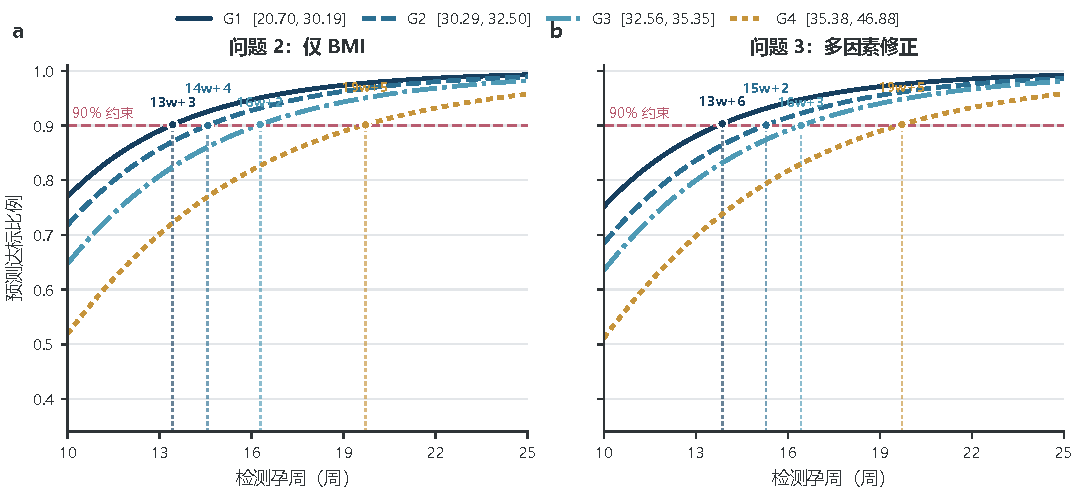
\includegraphics[width=0.97\textwidth]{q2_q3_reach_probability.pdf}
\caption{问题二、三各 BMI 组的预测达标概率}\label{fig:reach}
\end{figure}

图 \ref{fig:grouping} 直接展示连续 BMI 区间、组容量和推荐时点。问题二的中间两组较窄，是因为 30 至 35 的样本最密集且分位数变化较快；问题三第一组包含更多孕妇，但组 2、组 3 仍保留，用于隔离中高 BMI 人群的时点差异。该图把统计边界转化为可执行规则，避免只给切点而不说明样本支撑。

\begin{figure}[H]
\centering
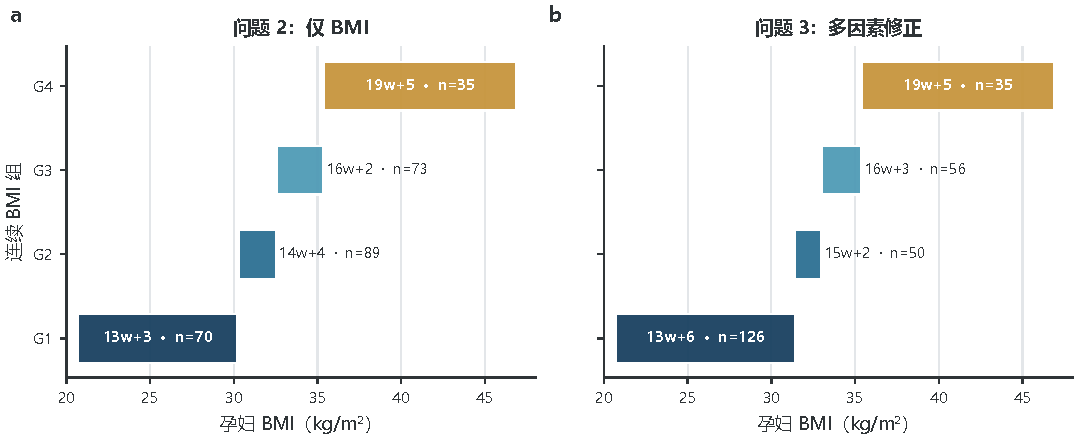
\includegraphics[width=0.95\textwidth]{grouping_decision_boundary.pdf}
\caption{连续 BMI 分组边界、组容量与推荐孕周}\label{fig:grouping}
\end{figure}

\subsection{问题四：女胎异常概率模型}

令 $y_i\in\{0,1\}$ 表示女胎第 $i$ 条记录是否异常，$x_i$ 为预处理后的特征向量。逻辑回归定义
\begin{equation}
p_i=P(y_i=1\mid x_i)=\frac{1}{1+\exp[-(\theta_0+x_i^\top\theta)]}.
\label{eq:logistic}
\end{equation}
在类别权重平衡和 $L_2$ 正则下，参数通过最小化
\begin{equation}
\min_{\theta_0,\theta}\left\{-\sum_{i=1}^{n}w_{y_i}\big[y_i\log p_i+(1-y_i)\log(1-p_i)\big]+\lambda\|\theta\|_2^2\right\}
\label{eq:logloss}
\end{equation}
求得。本文固定 $C=0.3$，即采用较强正则以降低小阳性样本下的系数波动。预测阈值取 0.5，不在全数据上二次搜索阈值，避免把验证标签用于调参。

基线规则为
\begin{equation}
\widehat y_i^{(Z)}=I\!\left(\max\{|Z_{13,i}|,|Z_{18,i}|,|Z_{21,i}|\}\ge3\right).
\label{eq:zrule}
\end{equation}
为了绘制 ROC 与 PR 曲线，将最大绝对 Z 值经中心在 3 的 Logistic 函数映射为连续分数，但阈值 0.5 与 $|Z|\ge3$ 完全对应。随机森林使用 500 棵树、每片叶的最小样本数为 5，并采用类别平衡抽样；直方图梯度提升使用 220 次迭代、最多 15 片叶和 $L_2$ 正则。三种学习模型共享同一五折 StratifiedGroupKFold，训练折与验证折的孕妇代码不重叠。

\subsubsection{特征组、正则化与折外预测}

候选特征分为四组。第一组是直接反映 13、18、21 号染色体偏离程度的 Z 值；第二组是 X 染色体浓度与 Z 值，用于补充女胎样本的性染色体信息；第三组是 GC 含量、总读段数、唯一比对读段数、比对比例、重复比例和过滤比例等测序质量指标；第四组是 BMI、年龄和检测孕周等个体背景。分组的目的不是分别训练四个模型，而是明确每类变量的含义和可获得时间。出生健康结局、男胎 Y 浓度以及由目标字段直接解析的变量均不进入特征集合。

逻辑回归对连续特征先做训练折内中位数填补和标准化。类别权重取各类样本数的反比，使 67 条异常记录不会在对数损失中被 538 条正常记录淹没。$L_2$ 正则把相关质量变量的系数共同收缩，降低小样本下某一变量获得极端权重的风险。选择 $C=0.3$ 是在预先给定的简洁正则范围内取较强收缩，并保持所有折使用相同设置；本文不在全部折外预测上再次试探大量 $C$ 和阈值组合，避免把最终验证结果变成隐含调参集。

折外预测按以下方式生成。先在孕妇层计算每名孕妇是否包含异常记录，以便在不拆分孕妇的前提下尽量平衡五折；第 $r$ 折只用其余四折估计缺失填充值、均值、标准差和模型参数，再对第 $r$ 折输出概率。五个验证折拼接后，每条记录恰有一个从未见过该孕妇的预测值。表中的 ROC-AUC、PR-AUC、混淆矩阵和 F1 全部由这组拼接概率计算，不是五个训练内指标的平均。这样做使各模型面对完全相同的测试记录，比较差异只来源于模型本身。

随机森林和梯度提升保留为结构不同的对照。森林通过多棵重抽样树平均，能够表示 Z 值或质量指标的非线性阈值；梯度提升逐步修正残差，能够形成更细的交互划分。如果二者显著超过线性概率模型，说明异常标签中存在重要非线性。实际结果却显示，树模型虽提高特异度，却明显降低召回率和 PR-AUC。这说明在异常样本较少且变量相关的条件下，更灵活的边界未转化为更好的少数类排序，正则化逻辑回归反而更稳健。

阈值 0.5 只用于给出一张固定混淆矩阵，ROC-AUC 与 PR-AUC 则利用全部可能阈值。对概率阈值 $t$，假阴性和假阳性数分别为
\begin{equation}
FN(t)=\sum_i I(y_i=1,p_i<t),\qquad
FP(t)=\sum_i I(y_i=0,p_i\ge t).
\label{eq:thresholderrors}
\end{equation}
降低 $t$ 通常提高召回率并降低特异度，反之亦然。题面没有提供两类错误的损失比，因而主文不以同一数据搜索一个看似精确的“最佳阈值”，而是报告固定阈值、完整曲线和错误结构，让使用者根据筛查目标选择工作点。

对验证集汇总混淆矩阵 $\{TN,FP,FN,TP\}$，主要指标定义为
\begin{align}
\mathrm{Recall}&=\frac{TP}{TP+FN},\qquad
\mathrm{Specificity}=\frac{TN}{TN+FP}, \label{eq:classmetric1}\\
\mathrm{Precision}&=\frac{TP}{TP+FP},\qquad
F_1=\frac{2\,\mathrm{Precision}\,\mathrm{Recall}}{\mathrm{Precision}+\mathrm{Recall}}.
\label{eq:classmetric2}
\end{align}
ROC-AUC 衡量随机异常记录获得更高分数的概率，PR-AUC 更关注少数阳性类，在本题中比准确率更有信息。Brier 分数用于检查概率误差，但由于类别权重改变了训练目标，未校准概率的 Brier 分数不作为唯一选模标准。

\begin{table}[H]
\centering
\caption{按孕妇分组的五折交叉验证结果}
\small
\begin{tabular}{lrrrrrr}
\toprule
模型 & ROC-AUC & PR-AUC & 精确率 & 召回率 & 特异度 & F1 \\
\midrule
分组逻辑回归 & 0.826 & 0.479 & 0.286 & 0.746 & 0.768 & 0.413 \\
随机森林 & 0.790 & 0.386 & 0.442 & 0.343 & 0.946 & 0.387 \\
直方图梯度提升 & 0.768 & 0.401 & 0.397 & 0.373 & 0.929 & 0.385 \\
传统 $|Z|\ge3$ & 0.479 & 0.109 & 0.089 & 0.060 & 0.924 & 0.071 \\
\bottomrule
\end{tabular}
\end{table}

逻辑回归的 ROC-AUC、PR-AUC、召回率和 F1 均为四种方法中最高，尽管精确率低于随机森林。赛题中的异常筛查更不能忽视漏检，因此选择逻辑回归作为主模型。其阈值 0.5 下混淆矩阵为 $TN=413$、$FP=125$、$FN=17$、$TP=50$。随机森林和梯度提升通过提高特异度减少误报，却把召回率降到 0.34--0.37，不符合本题对异常识别的主要关注。

\begin{figure}[H]
\centering
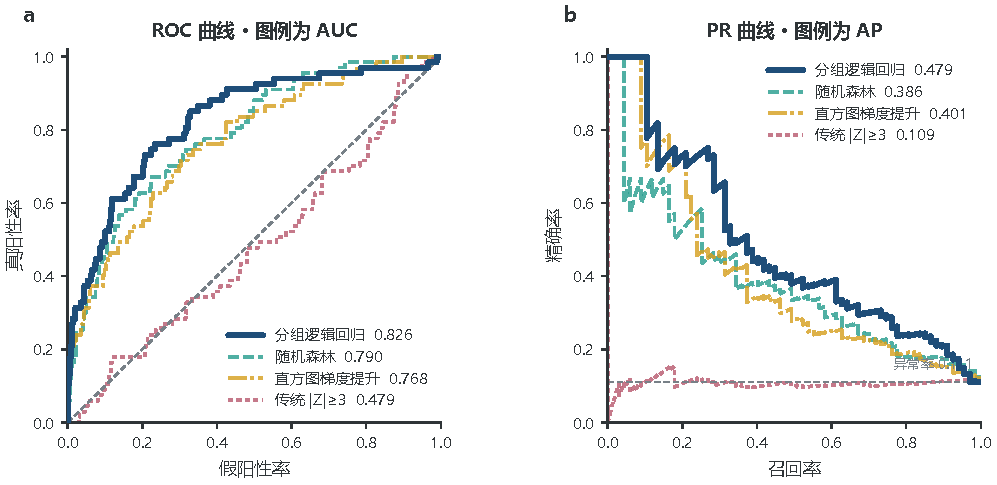
\includegraphics[width=0.97\textwidth]{q4_roc_pr.pdf}
\caption{女胎异常判定的 ROC 与 PR 曲线}\label{fig:rocpr}
\end{figure}

类别加权逻辑回归首先服务于少数类筛查，其原始输出是用于排序和阈值判定的筛查分数，不应未经检验直接解释为真实风险概率。为避免校准泄漏，本文在外层五折孕妇分组验证的每个训练折内，再进行四折孕妇分组预测，并只用内层折外分数拟合 Platt 映射；随后将该映射应用于外层未见孕妇。嵌套校准使 Brier 分数由 0.158 降至 0.081，等频八组的期望校准误差 ECE 为 0.035。汇总校准斜率仍为 1.55，说明内部概率误差虽明显缩小，仍需独立中心或后续批次重新校准。

图 \ref{fig:calibration} 左侧以 Wilson 95\% 区间展示校准后的预测概率和观察阳性率；右侧直接展示筛查分数阈值改变时召回率、特异度、精确率和 $F_1$ 的权衡。阈值 0.5 只是正文采用的固定工作点，不是从同一验证集搜索得到的临床最优值。降低阈值能减少漏检但显著增加假阳性，提高阈值则相反。

\begin{figure}[H]
\centering
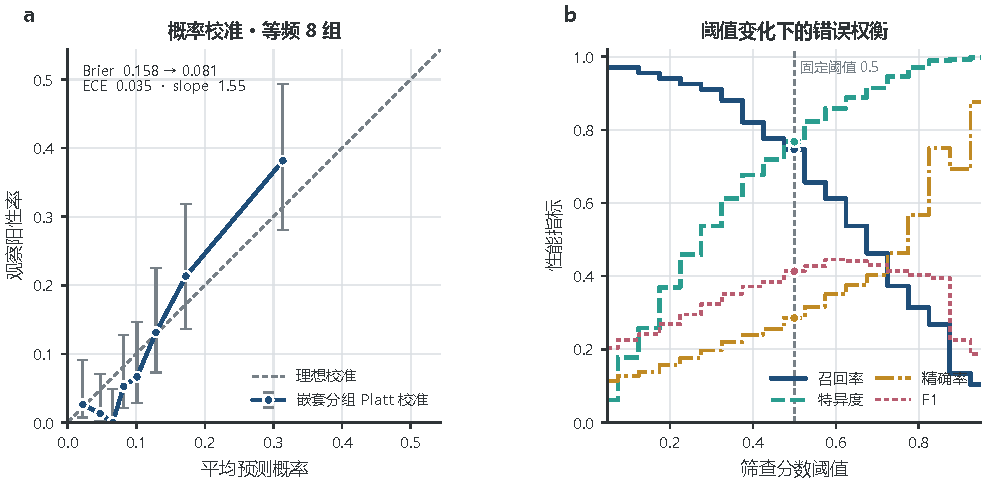
\includegraphics[width=0.97\textwidth]{q4_calibration_threshold.pdf}
\caption{女胎主模型的嵌套分组概率校准与阈值权衡}\label{fig:calibration}
\end{figure}

逻辑回归绝对系数较大的变量包括 13 号和 18 号染色体 GC 含量、21 号染色体 GC 含量、X 染色体浓度、年龄和 BMI。系数只表示在标准化与其他变量控制下的条件方向，不能解释为生物因果。图 \ref{fig:confusion} 左侧给出错误结构，右侧给出主要系数，有助于识别“高召回率伴随较多假阳性”的实际代价。

\begin{figure}[H]
\centering
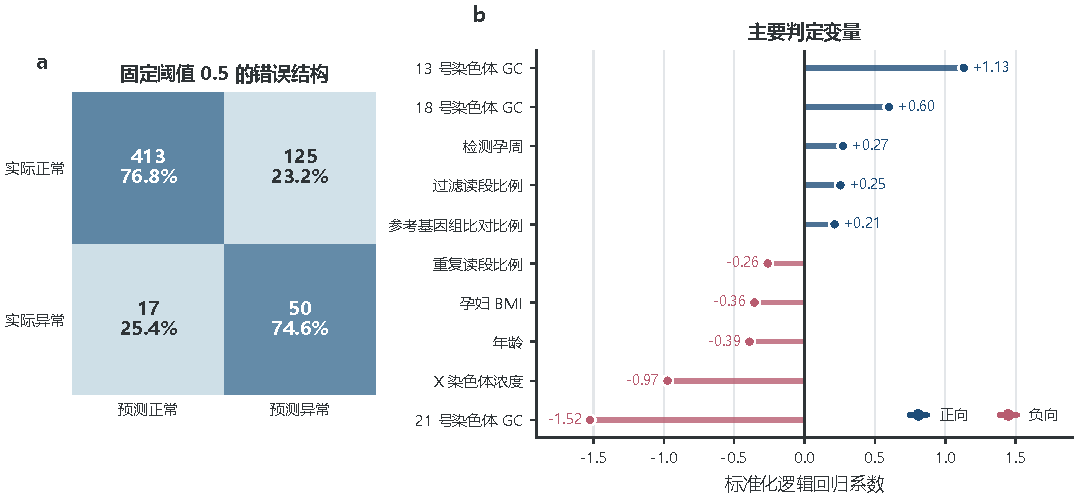
\includegraphics[width=0.92\textwidth]{q4_confusion_coefficients.pdf}
\caption{逻辑回归混淆矩阵与主要标准化系数}\label{fig:confusion}
\end{figure}

\section{模型检验}

\subsection{问题一的收敛、残差和组外预测}

混合模型成功收敛，随机截距方差和残差方差均为正。含随机效应的样本内拟合误差明显小于只含固定效应的误差，符合高 ICC 的预期。为了评价新孕妇而不是同一孕妇的新一次检测，五折验证使用孕妇代码分组；每一折在训练孕妇上拟合固定效应 OLS，再预测未见孕妇。得到 MAE 为 0.0270，$R^2=-0.036$。负的组外 $R^2$ 不是程序失败，而是说明固定人口变量对新孕妇单次浓度的预测弱于验证折均值基线；随机截距能解释已见孕妇，却不能在没有其既往测量时提前知道个体偏移。

图 \ref{fig:q1diag} 左侧以密度六边形和 LOWESS 曲线展示残差结构：残差总体围绕零分布，但低拟合值处离散更大；右侧 Q-Q 图主体接近直线，尾部少量点越出正态 95\% 包络。残差均值接近 0，标准差为 0.2142，5\% 和 95\% 分位数分别为 $-0.3604$ 和 0.3423。由此，固定效应显著性和总体方向较可信，但极端个体的点预测区间应比正态近似更宽。本文因此把问题一结论限定为总体关联，不给单名孕妇输出过度精确的浓度值。

\begin{figure}[H]
\centering
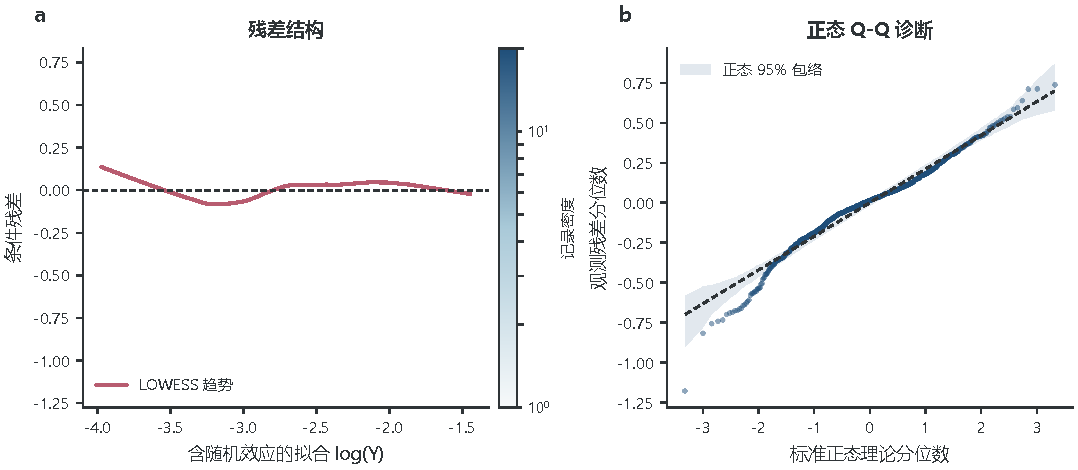
\includegraphics[width=0.96\textwidth]{q1_residual_diagnostic.pdf}
\caption{混合效应模型的拟合值--残差图与 Q-Q 图}\label{fig:q1diag}
\end{figure}

\subsection{问题二、三的可行性检查}

AFT 优化在两条路线和三个阈值情景下均成功。基准阈值下左删失 218 人、区间删失 42 人、右删失 7 人，三类样本都进入相应似然项，没有把右删失者删掉，也没有把左删失者固定在首次观测周。四个 BMI 组人数分别满足 $n_k\ge35$，所有推荐点的组平均达标概率都不低于 0.90，且推荐孕周位于题面 10 至 25 周窗口内。

常识检查有三项。第一，推荐时点随 BMI 总体推迟，与问题一的负 BMI 效应一致；若出现高 BMI 组更早且没有其他因素解释，应视为模型冲突。第二，4.5\% 阈值比 3.5\% 阈值严格，各组推荐时点均不应提前，实算结果满足该单调性。第三，多因素模型的 AIC 更高，正文没有把它包装为性能提升，而是保留为风险修正。三项检查分别约束方向、情景顺序和模型选择表述。

除方向检查外，还逐组核对概率可行性。推荐时点前一天记为 $t_k^- = t_k^*-1/7$，由最早性定义应满足 $\bar P_k(t_k^-)<0.90\le\bar P_k(t_k^*)$。如果前一天已经达到约束，则当前时点并非最早；如果推荐日仍低于约束，则网格搜索或分组汇总存在错误。两条路线的八个组均通过该检查。推荐日概率集中在 0.9003 至 0.9033，正是每天离散搜索跨过九成水平线的结果；它表明约束处于激活状态，而不是模型拥有异常精确的九成校准。

样本容量约束也需要结合尾部理解。最高 BMI 组均恰有 35 名孕妇，意味着其边界受到最小容量限制，不能把 35.38 解释为稳定的生理阈值。若把最小容量提高，尾组必须向较低 BMI 扩张；若降低容量，可能形成更晚但不稳定的小组。因此，表中 BMI 端点是“在给定容量和损失定义下的数据分界”，时点建议比小数端点更值得解释。对实际处于边界附近的孕妇，采用相邻两组中较晚时点可避免因 BMI 测量误差造成过早安排。

AFT 模型给出的是组平均达标概率，不保证组内每名孕妇都有九成概率。组平均机会约束符合题目要求的群体分组，但可能掩盖组内尾部风险。为检查这一点，动态分组直接最小化个体九成分位数的组内离差，使同组 $q_i$ 尽量接近；同时保留每组人数，防止均值由极少数低风险个体主导。若未来任务要求“组内至少九成孕妇各自达到某概率”，应把约束改成个体概率分位数或最坏情形约束，推荐时点将更保守。

\subsection{问题四的分组验证和不确定性}

五折划分同时满足“同一孕妇不跨折”和“各折尽量保持异常比例”。预测概率均为该记录所在验证折的折外输出，性能指标不使用训练内拟合值。传统 Z 规则不需要训练，但仍在同一记录集合上评价。逻辑回归的排序优势同时出现在 ROC-AUC 与 PR-AUC，避免只依赖单一指标。

在阳性率约为 0.111 的数据上，随机分类器的期望 PR-AUC 接近阳性率，而逻辑回归达到 0.479，约为基准水平的 4.3 倍。ROC-AUC 0.826 表示随机抽取一条异常和一条正常记录时，模型把异常赋予更高分数的概率约为 82.6\%；它衡量排序而非某一阈值下的命中率。固定阈值下，召回率 0.746 意味着 67 条异常记录中识别 50 条，特异度 0.768 意味着 538 条正常记录中正确排除 413 条。把这些比例还原成计数，可以避免只看 AUC 而忽略 125 条假阳性带来的进一步检查负担。

传统绝对 Z 值规则的特异度为 0.924，但召回率只有 0.060，说明它在附件标签下几乎只判定少量极端偏离记录。若单看准确率或特异度，可能错误地认为该规则较好；加入 PR-AUC、召回率和 F1 后，其少数类识别不足才显现。随机森林的精确率最高，但仅识别约三分之一异常；逻辑回归用更多假阳性换取了明显更高的异常覆盖。模型选择由筛查目标驱动，不是把所有指标简单平均。

为量化有限孕妇数量带来的波动，以 147 名孕妇为抽样单位做 500 次 Bootstrap。每次有放回抽取 147 个孕妇代码，并把被抽中孕妇的全部记录一并加入；若某次样本缺少一个类别则舍弃。对指标 $M$，百分位置信区间定义为
\begin{equation}
\mathrm{CI}_{0.95}(M)=\left[Q_{0.025}\{M^{*(b)}\},\ Q_{0.975}\{M^{*(b)}\}\right].
\label{eq:bootstrap}
\end{equation}

\begin{table}[H]
\centering
\caption{逻辑回归的孕妇分组 Bootstrap 不确定性}
\small
\begin{tabular}{lrrr}
\toprule
指标 & 点估计 & 95\%CI 下限 & 95\%CI 上限 \\
\midrule
ROC-AUC & 0.8259 & 0.7604 & 0.8781 \\
PR-AUC & 0.4791 & 0.3303 & 0.6191 \\
召回率 & 0.7463 & 0.6209 & 0.8483 \\
特异度 & 0.7677 & 0.7194 & 0.8102 \\
\bottomrule
\end{tabular}
\end{table}

PR-AUC 区间明显宽于 ROC-AUC，反映 67 条异常记录对精确率--召回率曲线的不确定性影响更大。即便在区间下限，ROC-AUC 仍高于随机排序；但这些区间来自附件内部重抽样，不能替代独立医院或独立批次的外部验证。

\begin{figure}[H]
\centering
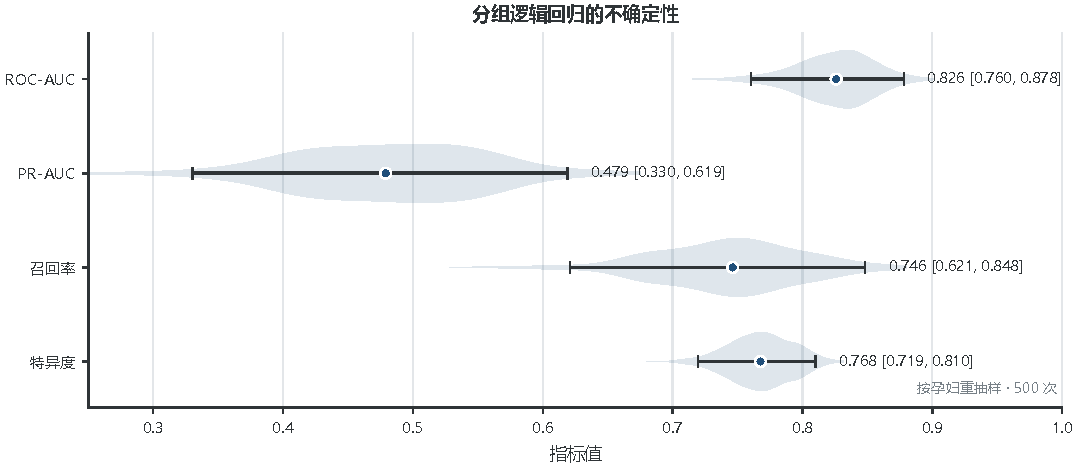
\includegraphics[width=0.78\textwidth]{q4_grouped_bootstrap_uncertainty.pdf}
\caption{女胎主模型性能的孕妇分组 Bootstrap 95\% 置信区间}\label{fig:bootstrap}
\end{figure}

\section{灵敏度与鲁棒性分析}

\subsection{达标阈值的测量误差传播}

题面把 4\% 作为可靠性的重要条件，但实验测量存在误差。本文不只在最终孕周上加减一个经验常数，而是分别以 3.5\%、4.0\%、4.5\% 重新判定每条记录、重新构造每名孕妇的删失区间、重新拟合 AFT 并重新搜索时点。设阈值为 $h$，基准为 $h_0=0.04$，第 $k$ 组时点变化定义为
\begin{equation}
\Delta_{k}(h)=7\,[t_k^*(h)-t_k^*(h_0)]\quad\text{天}.
\label{eq:sensitivity}
\end{equation}
全体路线和组别中的最大绝对变化为 17 天。低 BMI 组也会随阈值升高而推迟，但最高 BMI 组的绝对变化最大：问题二组 4 从 3.5\% 时的 17周3天推迟到 4.5\% 时的 21周6天。高 BMI 人群本就接近较低浓度区，阈值改变会使更多记录从达标转为未达标，故影响被放大。

\begin{figure}[H]
\centering
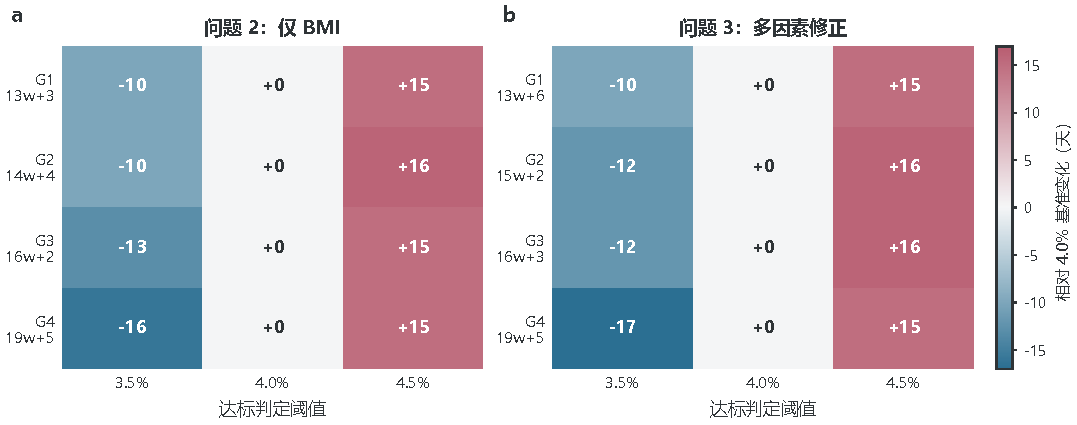
\includegraphics[width=0.88\textwidth]{q2_q3_error_sensitivity.pdf}
\caption{不同浓度阈值下推荐时点相对 4.0\% 基准的变化天数}\label{fig:sensitivity}
\end{figure}

阈值敏感性给出一个实际边界：推荐时点不是与实验误差无关的精确日期。对高 BMI 组，若实验室测量偏差或质量控制标准更严格，应预留约两周量级的时点不确定性；对低 BMI 组，变化相对较小。正文表格仍使用题面 4\% 基准，不把敏感性情景混入主结论。

\subsection{推荐时点的不确定性来源分解}

最终时点的不确定性并非单一标准误，而是由观测、抽样、模型和决策四个环节依次传递。第一类是浓度测量误差：同一孕周的测序深度、GC 偏差和过滤比例会使观测浓度围绕潜在值波动，从而改变某次记录是否越过阈值。第二类是区间观测误差：检测只在若干离散孕周发生，即使浓度无误，也只能把真实首次达标时点夹在相邻检测之间。第三类是样本波动：267 名男胎孕妇只是目标人群的一份样本，AFT 系数、BMI 边界和组内概率会随重新抽样变化。第四类是工作分布误差：对数正态假设提供单调概率曲线，但真实尾部若更厚，九成分位数可能偏移。第五类是决策离散误差：连续时点最终按天输出，概率跨过 0.90 的位置会有不超过一天的网格误差。

这些来源作用在不同层级，不能用一个阈值扰动代表全部不确定性。本文的 3.5、4.0、4.5 三个浓度情景主要覆盖测量判定和事件区间变化；AIC 比较主要反映协变量和分布复杂度；最小组容量控制边界的抽样脆弱性；按孕妇分组验证与 Bootstrap 则用于女胎分类的样本波动。由于附件缺少实验室重复测量的独立误差方差，无法把总时点方差精确分解为上述成分，因此不输出貌似完整但依据不足的单一置信区间。

从决策角度，可把基准推荐 $t_k^*(0.04)$ 与严格阈值推荐 $t_k^*(0.045)$ 组成一个稳健区间
\begin{equation}
\mathcal T_k^{\mathrm{rob}}=
\left[t_k^*(0.04),\ t_k^*(0.045)\right].
\label{eq:robustwindow}
\end{equation}
左端对应题面标准下的最早可行安排，右端对应更严格质量要求下的保守安排。该区间不是概率置信区间，而是阈值情景区间；它回答“质量标准变化时建议会移动到哪里”，不能回答“重复抽样时切点覆盖真值的概率”。明确两者差别可以防止把敏感性范围误写成统计置信区间。

最高 BMI 组的情景跨度最大，说明其建议对浓度判定最敏感。此时单纯再推迟检测虽能提高达标概率，却会减少后续处理时间。更合理的稳健策略是把等待和复检联合考虑：在基准时点进行首次检测，对质量未达标者按实验室规则复检，而不是所有人统一等待到严格情景的右端。附件没有复检成本、周转时间和临床处置代价，故本文不进一步计算成本最优策略，只给出可由现有数据支撑的概率边界。

女胎分类的不确定性则主要来自阳性样本少和孕妇内重复。Bootstrap 以孕妇而非记录重抽样，保留了每名孕妇记录数量和标签相关性。ROC-AUC 区间较窄而 PR-AUC 区间较宽，说明总体排序方向较稳定，但阳性预测的纯度更受样本组成影响。若新增数据，应优先增加独立异常孕妇和不同检测批次，而不是只为已有孕妇增加高度相似的重复记录；前者能更有效缩小少数类性能的不确定性。

\subsection{模型路线和极端情景的鲁棒性}

仅 BMI 与多因素 AFT 的最高 BMI 组边界和推荐时点均为 [35.38,46.88] 与 19周5天，说明最需要推迟的高 BMI 人群不依赖于复杂协变量组合。中间组边界存在变化，提示 31 至 35 BMI 区间更受年龄、身高和孕产史影响。对实际应用，可把最高组建议视为相对稳定，把中间组边界视为需要本地校准的软边界。

对数正态 AFT 的选择还可与两类替代方案比较。第一类是把“是否在某次检测达标”作为二元响应做 Logistic 回归，并把孕周作为自变量。该方案容易实现，也能得到随孕周变化的达标概率，但同一孕妇多次记录相关，且首次检测前已经达标的左删失信息会被拆成若干二元点；若再加入随机效应，模型虽能处理组内相关，却不能自然表示真实首次时点落在两次采样之间。第二类是只取首次观测达标周做普通回归。它舍弃始终未达标者，并把所有左删失者的上界当成精确值，偏差方向明确，故只适合作为粗略描述。

半参数区间删失比例风险模型可以减少分布假设，但其系数解释是风险比，求高条件分位数和在每天网格上计算个体达标概率更复杂；当样本只有 267 人、右删失仅 7 人时，尾部基准分布也可能不稳定。对数 Logistic 或 Weibull AFT 则保留直接的时间倍率解释，可作为后续替代分布。本文采用对数正态并非认定它是真实生理定律，而是因为其似然能统一三种删失、概率曲线单调、条件分位数有闭式表达，且与分组优化衔接自然。

分布稳健性的判断应关注最终决策而非只关注系数。即使两个 AFT 分布的某些系数不同，只要各 BMI 组的九成达标时点和顺序接近，决策就具有稳定性；反之，似然差异很小但高分位数相差数周时，尾部选择就至关重要。当前结果通过阈值情景和多因素路线验证了最高 BMI 组的稳定性，却没有完整比较所有工作分布，因此对中间组边界采取较弱表述。未来获得更大样本后，可按孕妇分组计算区间预测对数得分，并比较各分布的分位数覆盖率，再决定是否替换主模型。

动态分组同样存在替代目标。若使用组内推荐时点的绝对偏差，切点对极端 $q_i$ 更稳健；若使用最大组内差异，则会产生更均匀但更保守的组；若允许非连续分组，损失可能更低却难以形成 BMI 查表规则。本文的平方损失强调总体同质性，配合最小容量和连续性约束，适合竞赛题要求的分组建议。模型评价因此同时包含数值拟合、约束满足和规则可解释性，而不是只依据一个最小损失值。

问题一中 Spearman 相关系数为：孕周与 Y 浓度 0.0845，BMI 为 $-0.1550$，年龄为 $-0.1172$，体重为 $-0.1670$。这些边际相关方向与混合模型的孕周正效应和 BMI 负效应一致，但绝对值较小，说明单变量相关不能替代重复测量模型。混合模型显著性并非来自强线性相关，而是利用了全部纵向记录、控制变量和组内结构。

女胎分类的两种树模型特异度高于逻辑回归，但召回率显著下降；传统 Z 规则召回率仅 0.060。不同模型对“少误报”和“少漏报”的偏好差异很大。本文选择逻辑回归不是因为它在所有指标上占优，而是因为在不平衡筛查任务中，它提供最高的 PR-AUC、召回率和 F1，并且 ROC-AUC 也最高。分组 Bootstrap 进一步表明这一性能仍有明显区间宽度，不能把 0.826 写成无误差常数。

\section{结果解释}

\subsection{男胎浓度关系的含义}

孕周一次项显著为正，说明在附件范围内，随着妊娠进展，母体血液中可检测到的男胎 Y 染色体浓度总体升高。二次项为正，表示增长曲线存在一定上弯；但该形状只在 10 至 25 周观测范围内解释，不应向更早或更晚孕周外推。BMI 系数为负，说明体型增大与较低浓度相关，这与大样本 NIPT 研究的总体方向一致\cite{deng,rolnik}。

ICC=0.732 是问题一最重要的结构性结果之一。它说明同一孕妇的多次测量彼此相似，不同孕妇之间存在显著稳定差异。条件 $R^2$ 高而边际 $R^2$ 低，意味着已知某名孕妇的个体偏移后可解释较多变异，但仅凭常规人口变量预测从未见过的孕妇仍然困难。因此，群体模型适合制定分组策略，不适合替代个体复检和实验室质量判断。

\subsection{检测时点建议的含义}

问题二给出的 13周3天、14周4天、16周2天和19周5天不是“必须在这一天检测”，而是基于附件、4\% 阈值和 90\% 组平均达标约束得到的最早可行点。若检测资源允许个体化复检，可在更早时点检测并对未达标者复检；若目标是一次检测尽量获得可靠结果，则表中时点提供组层面的保守安排。高 BMI 组明显更晚，反映浓度分布整体下移，而非模型对高 BMI 人群施加人为惩罚。

问题三加入多因素后，第一组时点从 13周3天变为 13周6天，第二组从 14周4天变为 15周2天，第三组基本保持在 16 周附近，最高组不变。由于多因素 AIC 更高，不能据此宣称每个边界都更准确。更合适的解释是：BMI 提供稳定主分层，其他变量用于识别边界附近的异质性。若需实施，建议以问题二分组为主规则，在中间 BMI 区间参考问题三结果做风险提示。

\subsection{从模型输出到可执行规则}

模型落地时先确定规则层级。第一层是所有孕妇都能使用的 BMI 主规则：计算检测前最近一次可靠身高和体重对应的 BMI，按问题二四个连续区间确定基准时点。第二层是边界修正：若 BMI 位于两个组的分界附近，或年龄、身高、受孕方式和孕产史使问题三给出的条件分位数明显偏晚，则采用相邻两组中较晚的时点。第三层是检测后质量控制：抽血测序后若 Y 浓度未达题面标准或质量变量异常，进入复检流程，而不是回头改变检测前分组。三层分别使用决策前、决策辅助和检测后信息，保持时间顺序清楚。

BMI 自身存在测量误差。设测得 BMI 为 $B$、可能误差范围为 $[B-\delta_B,B+\delta_B]$。若整个区间落在同一组，只采用该组建议；若区间跨越分界，保守规则为
\begin{equation}
t_{\mathrm{use}}=max\{t_k^*: [B-\delta_B,B+\delta_B]\cap G_k\neq\varnothing\}.
\label{eq:bmierrorrule}
\end{equation}
这相当于在可能所属组中选较晚时点，避免因四舍五入或短期体重变化把孕妇错误地提前一组。对于远离边界的人群，规则不会额外推迟。题目没有给出 BMI 测量标准差，故 $\delta_B$ 应由实际测量流程确定，正文不任意指定数值。

推荐时点采用“周加天”表达而不使用两位小数孕周。例如 14周4天等于 $14+4/7$ 周，而不是 14.4 周；后者换算成天会产生约一天的偏差。执行时可以在推荐日之后的短窗口内预约，模型的机会约束在孕周增加时单调改善，因此延后少量时间不会降低预测达标概率。反之，提前预约应重新计算该日的组平均概率，不能只因日期接近就认为仍满足九成约束。

对于最高 BMI 组，19周5天已经明显晚于其他组。该建议的含义是附件样本中达到同一浓度可靠性需要更长等待，不意味着所有高 BMI 孕妇必须推迟到同一天。若实际流程允许早检加复检，可以在更早时点获得部分有效结果，并对未达标者再次采样；若资源紧张、希望提高一次成功率，则使用基准推荐更合适。两种策略对应不同成本结构，题目未提供采血成本、等待损失和复检周转时间，不能仅凭附件判断哪一种社会成本更低。

女胎异常判定也应作为筛查分流而非最终诊断。逻辑回归输出概率后，阈值 0.5 将记录分为“建议进一步检查”和“暂不触发二次筛查”两类。前者包含 50 条真阳性和 125 条假阳性，说明阳性输出必须进入后续检查；后者仍含 17 条假阴性，不能被表述为绝对正常。若实际场景把漏检代价设得更高，应降低概率阈值并接受更多二次筛查；若后续检查资源极有限，可提高阈值，但必须同时报告召回率下降。由此，模型提供的是可调分流工具，不是替代确诊的二元结论。

执行后的数据还应形成再校准闭环。每一批新孕妇都记录分组、推荐时点、实际采样周、Y 浓度是否达标、女胎预测概率和后续核验结果；定期按孕妇重新计算各组达标比例、PR-AUC、召回率和特异度。若某组在新数据中的达标比例持续低于 0.90，优先重新估计 AFT 参数和时点，而不是直接改动 BMI 边界；若分类概率整体偏高或偏低，则在独立校准样本上调整概率映射。该更新原则保持模型结构稳定，同时允许检测平台和人群分布变化后进行本地修正。

\subsection{女胎异常判定的含义}

传统 $|Z|\ge3$ 规则在附件上的召回率很低，说明“染色体的非整倍体”标签并非由单次三条常染色体绝对 Z 值完整生成。可能原因包括标签综合了更多染色体、重复检测、质量控制或人工判读信息。逻辑回归把 Z 值、X 染色体、GC 与读段质量、BMI、年龄和孕周联合起来，能复现更多标签结构，但它学习的是附件标签，不是确诊结果。

逻辑回归阈值 0.5 下每识别 50 条异常记录伴随 125 条假阳性，精确率只有 0.286。该结果不应被隐藏：提高召回率通常需要接受更多误报。若应用目标改为减少无效的后续检查，可提高阈值并牺牲召回率；若目标强调少漏检，则当前阈值更合适。题目没有提供不同错误的临床代价，本文不虚构代价权重，也不声称 0.5 是临床最优阈值。

\section{模型评价与改进}

\subsection{模型优点}

第一，模型结构与数据结构一致。问题一用随机截距表示重复测量，问题二、三用区间删失似然保留首次达标的不完全观测，问题四用孕妇分组验证和分组 Bootstrap 防止同一受试者泄漏。三处处理共享同一受试者层级，避免各问采用互相矛盾的独立性假设。

第二，时点决策具有明确目标函数和可行性约束。动态规划不是为增加算法复杂度，而是确保四个 BMI 区间连续、互斥、每组容量足够，并最小化个体条件高分位数的组内差异。推荐规则直接使用 90\% 达标机会约束，能够解释“为什么是这个孕周”，也能在阈值变化时重新计算。

第三，保留了不利结果。问题一组外 $R^2$ 略负，多因素 AFT 的 AIC 更高，传统 Z 规则与附件标签对应较弱，女胎 PR-AUC 置信区间较宽。保留这些结果能限制结论强度，防止把样本内拟合、复杂模型或单一指标误写成普遍优势。

第四，图表与主张一一对应。数据画像说明样本边界，关系图回答问题一，残差图检查假设，概率和分组图支撑问题二、三，敏感性图传播阈值误差，ROC/PR、混淆矩阵和 Bootstrap 图分别回答排序能力、错误结构与不确定性。图形不替代表格中的精确数值，而是帮助判断方向和边界。

\subsection{模型局限}

第一，样本外部代表性有限。附件 BMI 明显偏高，低 BMI 人群很少，动态分组的第一组跨度较大。任何面向一般孕妇的时点建议都需要在更宽 BMI 和更多中心数据上重新估计。本文没有外部验证集，因此所有性能区间都只表示附件内部不确定性。

第二，AFT 使用对数正态工作分布。区间删失处理比直接取首次观测周更合理，但若真实达标时间分布具有更重尾或不同形状，90\% 分位数会变化。可在后续比较 Weibull、对数 Logistic AFT 或半参数区间删失模型，并用交叉验证似然与分位数覆盖率选择分布。

第三，首次达到 4\% 的定义忽略了短期回落和实验重复误差。更完整的模型可把真实浓度视为潜在连续轨迹，把观测浓度视为带测量误差的重复值，再定义潜在轨迹越过阈值的时间。该联合纵向--事件模型需要实验室重复测量方差和更密集孕周数据，附件不足以稳定估计。

第四，女胎异常标签不是临床金标准。出生健康字段也不能直接充当金标准，因为其时间更晚、定义更宽。若获得羊水穿刺或核型确诊结果，应把确诊作为目标，附件筛查标签作为辅助变量；还应按医院、批次或时间做外部验证，检查概率校准和阈值迁移。

第五，逻辑回归特征间存在相关性，标准化系数会随特征集合变化。本文把系数用于解释模型方向而非生物因果。后续可采用稳定性选择、组 Lasso 或重复交叉验证，报告变量进入频率；若目标是临床风险概率，还需在独立校准集上做等距回归或 Platt 校准。

\subsection{可改进方向}

对问题一，可加入随机孕周斜率，使不同孕妇具有不同增长速度，并比较似然比、AIC 和收敛稳定性。当前每名孕妇观测次数有限，随机斜率可能导致方差估计贴边，因此未作为主模型。若未来记录更密集，可用样条固定效应或广义加性混合模型替代孕周二次项，减少外推形状限制。

对问题二、三，可用分层 Bootstrap 同时重抽样孕妇、重新拟合 AFT 和重新动态分组，得到切点与推荐孕周的置信区间。本文已对女胎分类做分组 Bootstrap，对时点则用阈值情景反映实验误差；两者覆盖的不确定性来源不同。完整切点 Bootstrap 计算量更大，但能区分采样波动与阈值误差。

对问题四，可根据题面或专家给出的假阴性/假阳性代价选择阈值。设假阴性代价为 $C_{FN}$、假阳性代价为 $C_{FP}$，验证集上的阈值可通过
\begin{equation}
t^*=\arg\min_t\{C_{FN}FN(t)+C_{FP}FP(t)\}
\label{eq:costthreshold}
\end{equation}
确定。但在没有可靠代价比时，任何“最优阈值”都依赖人为假设，因此本文只报告固定 0.5 阈值和完整指标，保留后续按场景选择的空间。

\section{结论}

问题一表明，男胎 Y 染色体浓度随孕周显著上升、随 BMI 显著下降；孕妇个体差异占据主要方差，故重复记录必须按孕妇建模和验证。问题二在 4\% 阈值、90\% 达标约束和每组至少 35 人条件下，得到四个连续 BMI 区间，对应推荐时点为 13周3天、14周4天、16周2天和19周5天。问题三加入年龄、身高、受孕方式和孕产史后得到 13周6天、15周2天、16周3天和19周5天，但 AIC 没有改善，因此仅作为风险修正；阈值从 3.5\% 调至 4.5\% 时，时点最多改变 17 天。

问题四中，按孕妇分组五折验证的逻辑回归取得 ROC-AUC 0.826、PR-AUC 0.479、召回率 0.746 和特异度 0.768，优于随机森林、梯度提升和传统 Z 阈值；分组 Bootstrap 表明 ROC-AUC 的 95\% 区间为 $[0.760,0.878]$。这些结果能回答赛题中的群体分组和异常判定，但不能直接替代临床复检、确诊或实验室质量控制。模型的适用范围以附件人群、字段口径和检测平台为边界。

四问的共同结论是：NIPT 决策不能只依赖单次记录或单一阈值。男胎时点需要同时处理个体差异、未被精确观察的首次达标时间与分组容量；女胎判定需要同时处理少数类、测序质量和同一孕妇重复检测。本文用孕妇代码统一这些统计层级，使系数检验、时点优化、折外评价和不确定性估计针对同一个独立单位。对于附件数据，BMI 是最稳定、最便于执行的时点分层变量，其他检测前因素适合修正边界而不足以替代主规则；女胎逻辑回归则适合做高召回的风险分流，但其较低精确率要求后续检查。若检测平台、人群 BMI 分布或标签定义发生变化，应重新估计参数和概率，不直接移植本文数值。

{\small
\begin{thebibliography}{10}
\setlength{\itemsep}{0.2em}
\bibitem{problem} 全国大学生数学建模竞赛组委会. 2025 年高教社杯全国大学生数学建模竞赛赛题, 2025.
\bibitem{deng} Deng C, et al. Maternal and fetal factors influencing fetal fraction: a retrospective analysis of 153,306 pregnant women undergoing noninvasive prenatal screening. 2023. PMID: 37114008.
\bibitem{gazdarica} Gazdarica J, et al. Insights into non-informative results from non-invasive prenatal screening through gestational age, maternal BMI, and age analyses. 2024. PMID: 38452118.
\bibitem{rolnik} Rolnik DL, et al. Influence of Body Mass Index on Fetal Fraction Increase With Gestation and Cell-Free DNA Test Failure. 2018. PMID: 29995742.
\bibitem{zhang} Zhang X, et al. Z-score accuracy of noninvasive prenatal testing for fetal trisomies 13, 18 and 21 at a single center. 2021. PMID: 33480032.
\bibitem{laird} Laird NM, Ware JH. Random-effects models for longitudinal data. Biometrics, 1982, 38(4): 963--974.
\bibitem{klein} Klein JP, Moeschberger ML. Survival Analysis: Techniques for Censored and Truncated Data. Springer, 2003.
\bibitem{breiman} Breiman L. Random Forests. Machine Learning, 2001, 45: 5--32.
\bibitem{sklearn} Pedregosa F, et al. Scikit-learn: Machine Learning in Python. Journal of Machine Learning Research, 2011, 12: 2825--2830.
\end{thebibliography}
\par\smallskip
\appendix
{\footnotesize\noindent\textbf{复现说明：}在项目根目录运行 \texttt{python src/run\_all.py}；随机种子为 2025，交叉验证、嵌套校准与 Bootstrap 均按孕妇分组。脚本可重建清洗数据、结果表、三格式图形和结构化摘要。}
}

\end{document}
